\PassOptionsToPackage{unicode=true}{hyperref} % options for packages loaded elsewhere
\PassOptionsToPackage{hyphens}{url}
%
\documentclass[]{article}
\usepackage{lmodern}
\usepackage{amssymb,amsmath}
\usepackage{ifxetex,ifluatex}
\usepackage{fixltx2e} % provides \textsubscript
\ifnum 0\ifxetex 1\fi\ifluatex 1\fi=0 % if pdftex
  \usepackage[T1]{fontenc}
  \usepackage[utf8]{inputenc}
  \usepackage{textcomp} % provides euro and other symbols
\else % if luatex or xelatex
  \usepackage{unicode-math}
  \defaultfontfeatures{Ligatures=TeX,Scale=MatchLowercase}
\fi
% use upquote if available, for straight quotes in verbatim environments
\IfFileExists{upquote.sty}{\usepackage{upquote}}{}
% use microtype if available
\IfFileExists{microtype.sty}{%
\usepackage[]{microtype}
\UseMicrotypeSet[protrusion]{basicmath} % disable protrusion for tt fonts
}{}
\IfFileExists{parskip.sty}{%
\usepackage{parskip}
}{% else
\setlength{\parindent}{0pt}
\setlength{\parskip}{6pt plus 2pt minus 1pt}
}
\usepackage{hyperref}
\hypersetup{
            pdftitle={Day 10 - Categorical Variables and Nested F Tests},
            pdfauthor={SDS 291},
            pdfborder={0 0 0},
            breaklinks=true}
\urlstyle{same}  % don't use monospace font for urls
\usepackage[margin=1in]{geometry}
\usepackage{color}
\usepackage{fancyvrb}
\newcommand{\VerbBar}{|}
\newcommand{\VERB}{\Verb[commandchars=\\\{\}]}
\DefineVerbatimEnvironment{Highlighting}{Verbatim}{commandchars=\\\{\}}
% Add ',fontsize=\small' for more characters per line
\usepackage{framed}
\definecolor{shadecolor}{RGB}{248,248,248}
\newenvironment{Shaded}{\begin{snugshade}}{\end{snugshade}}
\newcommand{\AlertTok}[1]{\textcolor[rgb]{0.94,0.16,0.16}{#1}}
\newcommand{\AnnotationTok}[1]{\textcolor[rgb]{0.56,0.35,0.01}{\textbf{\textit{#1}}}}
\newcommand{\AttributeTok}[1]{\textcolor[rgb]{0.77,0.63,0.00}{#1}}
\newcommand{\BaseNTok}[1]{\textcolor[rgb]{0.00,0.00,0.81}{#1}}
\newcommand{\BuiltInTok}[1]{#1}
\newcommand{\CharTok}[1]{\textcolor[rgb]{0.31,0.60,0.02}{#1}}
\newcommand{\CommentTok}[1]{\textcolor[rgb]{0.56,0.35,0.01}{\textit{#1}}}
\newcommand{\CommentVarTok}[1]{\textcolor[rgb]{0.56,0.35,0.01}{\textbf{\textit{#1}}}}
\newcommand{\ConstantTok}[1]{\textcolor[rgb]{0.00,0.00,0.00}{#1}}
\newcommand{\ControlFlowTok}[1]{\textcolor[rgb]{0.13,0.29,0.53}{\textbf{#1}}}
\newcommand{\DataTypeTok}[1]{\textcolor[rgb]{0.13,0.29,0.53}{#1}}
\newcommand{\DecValTok}[1]{\textcolor[rgb]{0.00,0.00,0.81}{#1}}
\newcommand{\DocumentationTok}[1]{\textcolor[rgb]{0.56,0.35,0.01}{\textbf{\textit{#1}}}}
\newcommand{\ErrorTok}[1]{\textcolor[rgb]{0.64,0.00,0.00}{\textbf{#1}}}
\newcommand{\ExtensionTok}[1]{#1}
\newcommand{\FloatTok}[1]{\textcolor[rgb]{0.00,0.00,0.81}{#1}}
\newcommand{\FunctionTok}[1]{\textcolor[rgb]{0.00,0.00,0.00}{#1}}
\newcommand{\ImportTok}[1]{#1}
\newcommand{\InformationTok}[1]{\textcolor[rgb]{0.56,0.35,0.01}{\textbf{\textit{#1}}}}
\newcommand{\KeywordTok}[1]{\textcolor[rgb]{0.13,0.29,0.53}{\textbf{#1}}}
\newcommand{\NormalTok}[1]{#1}
\newcommand{\OperatorTok}[1]{\textcolor[rgb]{0.81,0.36,0.00}{\textbf{#1}}}
\newcommand{\OtherTok}[1]{\textcolor[rgb]{0.56,0.35,0.01}{#1}}
\newcommand{\PreprocessorTok}[1]{\textcolor[rgb]{0.56,0.35,0.01}{\textit{#1}}}
\newcommand{\RegionMarkerTok}[1]{#1}
\newcommand{\SpecialCharTok}[1]{\textcolor[rgb]{0.00,0.00,0.00}{#1}}
\newcommand{\SpecialStringTok}[1]{\textcolor[rgb]{0.31,0.60,0.02}{#1}}
\newcommand{\StringTok}[1]{\textcolor[rgb]{0.31,0.60,0.02}{#1}}
\newcommand{\VariableTok}[1]{\textcolor[rgb]{0.00,0.00,0.00}{#1}}
\newcommand{\VerbatimStringTok}[1]{\textcolor[rgb]{0.31,0.60,0.02}{#1}}
\newcommand{\WarningTok}[1]{\textcolor[rgb]{0.56,0.35,0.01}{\textbf{\textit{#1}}}}
\usepackage{graphicx,grffile}
\makeatletter
\def\maxwidth{\ifdim\Gin@nat@width>\linewidth\linewidth\else\Gin@nat@width\fi}
\def\maxheight{\ifdim\Gin@nat@height>\textheight\textheight\else\Gin@nat@height\fi}
\makeatother
% Scale images if necessary, so that they will not overflow the page
% margins by default, and it is still possible to overwrite the defaults
% using explicit options in \includegraphics[width, height, ...]{}
\setkeys{Gin}{width=\maxwidth,height=\maxheight,keepaspectratio}
\setlength{\emergencystretch}{3em}  % prevent overfull lines
\providecommand{\tightlist}{%
  \setlength{\itemsep}{0pt}\setlength{\parskip}{0pt}}
\setcounter{secnumdepth}{0}
% Redefines (sub)paragraphs to behave more like sections
\ifx\paragraph\undefined\else
\let\oldparagraph\paragraph
\renewcommand{\paragraph}[1]{\oldparagraph{#1}\mbox{}}
\fi
\ifx\subparagraph\undefined\else
\let\oldsubparagraph\subparagraph
\renewcommand{\subparagraph}[1]{\oldsubparagraph{#1}\mbox{}}
\fi

% set default figure placement to htbp
\makeatletter
\def\fps@figure{htbp}
\makeatother


\title{Day 10 - Categorical Variables and Nested F Tests}
\author{SDS 291}
\date{February 26, 2020}

\begin{document}
\maketitle

\hypertarget{birthweight-and-parental-smoking}{%
\subsection{Birthweight and parental
smoking}\label{birthweight-and-parental-smoking}}

Using data from the mosaic package. Birth weight, date, and gestational
period collected as part of the Child Health and Development Studies
from Oakland, CA in 1961 and 1962; we're working with a sample of 1,263
babies and their parents. The study is
\href{http://www.chdstudies.org/index.php}{still ongoing}, now following
its 3rd generation.

\begin{itemize}
\tightlist
\item
  Response variable

  \begin{itemize}
  \tightlist
  \item
    \texttt{wt}: birth weight (in ounces)
  \end{itemize}
\item
  Explanatory Variable(s)

  \begin{itemize}
  \tightlist
  \item
    \texttt{smoke}: smoke does mother smoke? 0=never, 1=smokes now,
    2=until current pregnancy, 3=once did, not now
  \item
    \texttt{age}: mother's age in years at termination of pregnancy
  \end{itemize}
\end{itemize}

Bring in the data

\begin{Shaded}
\begin{Highlighting}[]
\KeywordTok{require}\NormalTok{(mosaic)}
\KeywordTok{require}\NormalTok{(tidyverse)}
\KeywordTok{require}\NormalTok{(magrittr)}
\KeywordTok{data}\NormalTok{(}\StringTok{"Gestation"}\NormalTok{)}
\NormalTok{Gestation<-Gestation }\OperatorTok\StringTok{ }\KeywordTok{filter}\NormalTok{(}\OperatorTok{!}\KeywordTok{is.na}\NormalTok{(smoke), }\OperatorTok{!}\KeywordTok{is.na}\NormalTok{(wt))}
\end{Highlighting}
\end{Shaded}

Now fit the model: \[bithweight=\beta_0+\beta_1 smoke+ \epsilon\]

\begin{Shaded}
\begin{Highlighting}[]
\NormalTok{m_quant<-}\KeywordTok{lm}\NormalTok{(wt}\OperatorTok{~}\NormalTok{smoke, }\DataTypeTok{data=}\NormalTok{Gestation)}
\KeywordTok{summary}\NormalTok{(m_quant)}
\end{Highlighting}
\end{Shaded}

\begin{verbatim}
## 
## Call:
## lm(formula = wt ~ smoke, data = Gestation)
## 
## Residuals:
##     Min      1Q  Median      3Q     Max 
## -64.855 -10.855   0.274  11.145  56.145 
## 
## Coefficients:
##             Estimate Std. Error t value Pr(>|t|)    
## (Intercept) 119.8553     0.6949  172.48   <2e-16 ***
## smoke        -0.4198     0.5749   -0.73    0.465    
## ---
## Signif. codes:  0 '***' 0.001 '**' 0.01 '*' 0.05 '.' 0.1 ' ' 1
## 
## Residual standard error: 18.21 on 1224 degrees of freedom
## Multiple R-squared:  0.0004353,  Adjusted R-squared:  -0.0003814 
## F-statistic: 0.533 on 1 and 1224 DF,  p-value: 0.4655
\end{verbatim}

\#\#\#\#How do you interpret the coefficient for \texttt{smoke}?

\textbf{Answer}: Like the example with gender above, this is treating
\texttt{smoke} as a quantitative variable. So it can be interpreted as a
1-unit increase in smoking status is associated with a 0.42lb lighter
child at birth, on average in the population.

\newpage

\hypertarget{what-if-smoking-status-were-a-categorical-variable}{%
\subsection{What if smoking status were a categorical
variable?}\label{what-if-smoking-status-were-a-categorical-variable}}

\#\#\#R uses \texttt{factor} variables to indicate categorical
variables.

You could make a new variable \texttt{smoke\_factor} with the same
values as \texttt{smoke} but where \texttt{R} knows the variable should
be formatted as a factor.

\begin{Shaded}
\begin{Highlighting}[]
\NormalTok{Gestation<-Gestation }\OperatorTok
\StringTok{  }\KeywordTok{mutate}\NormalTok{(}\DataTypeTok{smoke_factor=}\KeywordTok{as.factor}\NormalTok{(smoke))}
\NormalTok{m_cat1<-}\KeywordTok{lm}\NormalTok{(wt}\OperatorTok{~}\NormalTok{smoke_factor, }\DataTypeTok{data=}\NormalTok{Gestation)}
\KeywordTok{summary}\NormalTok{(m_cat1)}
\end{Highlighting}
\end{Shaded}

\begin{verbatim}
## 
## Call:
## lm(formula = wt ~ smoke_factor, data = Gestation)
## 
## Residuals:
##    Min     1Q Median     3Q    Max 
## -67.78 -11.11   0.89  11.22  53.22 
## 
## Coefficients:
##               Estimate Std. Error t value Pr(>|t|)    
## (Intercept)   122.7776     0.7583 161.904  < 2e-16 ***
## smoke_factor1  -8.6681     1.1052  -7.843 9.53e-15 ***
## smoke_factor2   0.3066     1.9668   0.156    0.876    
## smoke_factor3   1.6593     1.9006   0.873    0.383    
## ---
## Signif. codes:  0 '***' 0.001 '**' 0.01 '*' 0.05 '.' 0.1 ' ' 1
## 
## Residual standard error: 17.69 on 1222 degrees of freedom
## Multiple R-squared:  0.05823,    Adjusted R-squared:  0.05592 
## F-statistic: 25.19 on 3 and 1222 DF,  p-value: 8.196e-16
\end{verbatim}

\hypertarget{what-is-the-average-expected-birthweight-of-a-child-whose-mother-never-smoked}{%
\paragraph{What is the average expected birthweight of a child whose
mother never
smoked?}\label{what-is-the-average-expected-birthweight-of-a-child-whose-mother-never-smoked}}

\textbf{Answer}: The average expected birthweight of a child whose
mother never smoked is 122.78 ounces.

\hypertarget{interpret-the-coefficient-for-smoke_factor1.}{%
\paragraph{\texorpdfstring{Interpret the coefficient for
\texttt{smoke\_factor1}.}{Interpret the coefficient for smoke\_factor1.}}\label{interpret-the-coefficient-for-smoke_factor1.}}

\textbf{Answer}: The coefficient for \texttt{smoke\_factor1} reflects
the difference in the average expected birthweight of a child whose
mother is a current smoker to a child whose mother never smoked.
Specifically, a child born to a mother who is a current smoker will
weigh 8.67 ounces lighter at birth than a child born to a mother who
never smoked, on average in this population. This -8.67 ounce difference
in birthweight between current and never smoker mothers is
statisticially significant from 0 since the t-statistic (-7.8) is below
the critical value of 1.96, and the p-value (9.53e-15) is
\textless{}0.05.

\hypertarget{interpret-the-coefficient-for-smoke_factor2.}{%
\paragraph{\texorpdfstring{Interpret the coefficient for
\texttt{smoke\_factor2}.}{Interpret the coefficient for smoke\_factor2.}}\label{interpret-the-coefficient-for-smoke_factor2.}}

\textbf{Answer}: The coefficient for \texttt{smoke\_factor2} reflects
the difference in the average expected birthweight of a child whose
mother who smoked until pregnancy to a mother who never smoked. A child
of a woman who smoked prior to pregnancy weighed, on average, .3066
ounces more than a child of a never smoker mother in this population.
This difference was not statistically signigicantly different from 0,
since the t-statistic (0.156) was \textless{}1.96 and the p-value
(0.876) was \textgreater{}0.05.

It's hard to keep the values of these levels straight. Especially if you
had multiple factor variables. Instead, you might make the factor levels
be something more conceptually understandable.

\begin{Shaded}
\begin{Highlighting}[]
\NormalTok{Gestation<-Gestation }\OperatorTok
\StringTok{  }\KeywordTok{mutate}\NormalTok{(}\DataTypeTok{smoke_cat=}\KeywordTok{as.factor}\NormalTok{(}\KeywordTok{if_else}\NormalTok{(smoke}\OperatorTok{==}\DecValTok{0}\NormalTok{,}\StringTok{"never smoker"}\NormalTok{,}
                             \KeywordTok{if_else}\NormalTok{(smoke}\OperatorTok{==}\DecValTok{1}\NormalTok{,}\StringTok{"current smoker"}\NormalTok{,}
                             \KeywordTok{if_else}\NormalTok{(smoke}\OperatorTok{==}\DecValTok{2}\NormalTok{,}\StringTok{"pre-pregnancy smoker"}\NormalTok{,}
                             \KeywordTok{if_else}\NormalTok{(smoke}\OperatorTok{==}\DecValTok{3}\NormalTok{,}\StringTok{"other former smoker"}\NormalTok{,}\StringTok{"NA"}\NormalTok{))))}
\NormalTok{                   )}
\NormalTok{        )}
\KeywordTok{tally}\NormalTok{(}\OperatorTok{~}\NormalTok{smoke_cat, }\DataTypeTok{data=}\NormalTok{Gestation)}
\end{Highlighting}
\end{Shaded}

\begin{verbatim}
## smoke_cat
##       current smoker         never smoker  other former smoker 
##                  484                  544                  103 
## pre-pregnancy smoker 
##                   95
\end{verbatim}

\begin{Shaded}
\begin{Highlighting}[]
\NormalTok{smoke_factor_labels<-}\KeywordTok{lm}\NormalTok{(wt}\OperatorTok{~}\KeywordTok{I}\NormalTok{(smoke_cat), }\DataTypeTok{data=}\NormalTok{Gestation)}
\KeywordTok{summary}\NormalTok{(smoke_factor_labels)}
\end{Highlighting}
\end{Shaded}

\begin{verbatim}
## 
## Call:
## lm(formula = wt ~ I(smoke_cat), data = Gestation)
## 
## Residuals:
##    Min     1Q Median     3Q    Max 
## -67.78 -11.11   0.89  11.22  53.22 
## 
## Coefficients:
##                                  Estimate Std. Error t value Pr(>|t|)    
## (Intercept)                       114.109      0.804 141.933  < 2e-16 ***
## I(smoke_cat)never smoker            8.668      1.105   7.843 9.53e-15 ***
## I(smoke_cat)other former smoker    10.327      1.919   5.381 8.88e-08 ***
## I(smoke_cat)pre-pregnancy smoker    8.975      1.985   4.522 6.73e-06 ***
## ---
## Signif. codes:  0 '***' 0.001 '**' 0.01 '*' 0.05 '.' 0.1 ' ' 1
## 
## Residual standard error: 17.69 on 1222 degrees of freedom
## Multiple R-squared:  0.05823,    Adjusted R-squared:  0.05592 
## F-statistic: 25.19 on 3 and 1222 DF,  p-value: 8.196e-16
\end{verbatim}

\hypertarget{what-is-the-average-expected-birthweight-of-a-child-whose-mother-never-smoked-1}{%
\paragraph{What is the average expected birthweight of a child whose
mother never
smoked?}\label{what-is-the-average-expected-birthweight-of-a-child-whose-mother-never-smoked-1}}

\textbf{Answer}: The average expected birthweight of a child whose
mother never smoked was 122.78 ounces (114.109+8.668).

\hypertarget{what-is-the-average-expected-birthweight-of-a-child-whose-mother-was-a-current-smoker}{%
\paragraph{What is the average expected birthweight of a child whose
mother was a current
smoker?}\label{what-is-the-average-expected-birthweight-of-a-child-whose-mother-was-a-current-smoker}}

\textbf{Answer}: The average expected birthweight of a child whose
mother was a current smoker was 114.11 ounces.

\hypertarget{how-to-get-the-right-reference-group}{%
\subsection{How to get the right reference
group?}\label{how-to-get-the-right-reference-group}}

You can tell \texttt{R} what you want the reference group to be with
\texttt{relevel()} function.

\begin{Shaded}
\begin{Highlighting}[]
\NormalTok{Gestation}\OperatorTok{$}\NormalTok{smoke_cat<-}\KeywordTok{relevel}\NormalTok{(Gestation}\OperatorTok{$}\NormalTok{smoke_cat, }\DataTypeTok{ref =} \StringTok{"never smoker"}\NormalTok{)}
\end{Highlighting}
\end{Shaded}

But \emph{the better option} is to make dummy/indicator variables for
each of the categories.

\begin{Shaded}
\begin{Highlighting}[]
\NormalTok{Gestation<-Gestation }\OperatorTok
\StringTok{  }\KeywordTok{mutate}\NormalTok{(}
    \DataTypeTok{smoke_nev=}\KeywordTok{if_else}\NormalTok{(smoke}\OperatorTok{==}\DecValTok{0}\NormalTok{,}\DecValTok{1}\NormalTok{,}\DecValTok{0}\NormalTok{),}
    \DataTypeTok{smoke_cur=}\KeywordTok{if_else}\NormalTok{(smoke}\OperatorTok{==}\DecValTok{1}\NormalTok{,}\DecValTok{1}\NormalTok{,}\DecValTok{0}\NormalTok{),}
    \DataTypeTok{smoke_pre=}\KeywordTok{if_else}\NormalTok{(smoke}\OperatorTok{==}\DecValTok{2}\NormalTok{,}\DecValTok{1}\NormalTok{,}\DecValTok{0}\NormalTok{),}
    \DataTypeTok{smoke_fmr=}\KeywordTok{if_else}\NormalTok{(smoke}\OperatorTok{==}\DecValTok{3}\NormalTok{,}\DecValTok{1}\NormalTok{,}\DecValTok{0}\NormalTok{)}
\NormalTok{  )}
\KeywordTok{tally}\NormalTok{(}\KeywordTok{c}\NormalTok{(}\StringTok{"smoke_nev"}\NormalTok{, }\StringTok{"smoke_cur"}\NormalTok{, }\StringTok{"smoke_pre"}\NormalTok{, }\StringTok{"smoke_fmr"}\NormalTok{), }\DataTypeTok{data=}\NormalTok{Gestation)}
\end{Highlighting}
\end{Shaded}

\begin{verbatim}
## X
## smoke_cur smoke_fmr smoke_nev smoke_pre 
##         1         1         1         1
\end{verbatim}

\begin{Shaded}
\begin{Highlighting}[]
\NormalTok{smoke_indicators<-}\KeywordTok{lm}\NormalTok{(wt}\OperatorTok{~}\NormalTok{smoke_nev}\OperatorTok{+}\NormalTok{smoke_cur}\OperatorTok{+}\NormalTok{smoke_pre}\OperatorTok{+}\NormalTok{smoke_fmr, }\DataTypeTok{data=}\NormalTok{Gestation)}
\KeywordTok{summary}\NormalTok{(smoke_indicators)}
\end{Highlighting}
\end{Shaded}

\begin{verbatim}
## 
## Call:
## lm(formula = wt ~ smoke_nev + smoke_cur + smoke_pre + smoke_fmr, 
##     data = Gestation)
## 
## Residuals:
##    Min     1Q Median     3Q    Max 
## -67.78 -11.11   0.89  11.22  53.22 
## 
## Coefficients: (1 not defined because of singularities)
##             Estimate Std. Error t value Pr(>|t|)    
## (Intercept)  124.437      1.743  71.401  < 2e-16 ***
## smoke_nev     -1.659      1.901  -0.873    0.383    
## smoke_cur    -10.327      1.919  -5.381 8.88e-08 ***
## smoke_pre     -1.353      2.516  -0.538    0.591    
## smoke_fmr         NA         NA      NA       NA    
## ---
## Signif. codes:  0 '***' 0.001 '**' 0.01 '*' 0.05 '.' 0.1 ' ' 1
## 
## Residual standard error: 17.69 on 1222 degrees of freedom
## Multiple R-squared:  0.05823,    Adjusted R-squared:  0.05592 
## F-statistic: 25.19 on 3 and 1222 DF,  p-value: 8.196e-16
\end{verbatim}

\newpage

\hypertarget{what-does-the-anova-table-tell-us}{%
\subsection{What does the ANOVA table tell
us?}\label{what-does-the-anova-table-tell-us}}

\begin{Shaded}
\begin{Highlighting}[]
\KeywordTok{anova}\NormalTok{(smoke_indicators)}
\end{Highlighting}
\end{Shaded}

\begin{verbatim}
## Analysis of Variance Table
## 
## Response: wt
##             Df Sum Sq Mean Sq F value    Pr(>F)    
## smoke_nev    1  10385 10385.4  33.197 1.053e-08 ***
## smoke_cur    1  13162 13162.3  42.074 1.274e-10 ***
## smoke_pre    1     90    90.4   0.289    0.5909    
## Residuals 1222 382290   312.8                      
## ---
## Signif. codes:  0 '***' 0.001 '**' 0.01 '*' 0.05 '.' 0.1 ' ' 1
\end{verbatim}

\hypertarget{whats-the-msmodel}{%
\paragraph{What's the MSModel?}\label{whats-the-msmodel}}

The MSModel is 7879.333 ((23399.5+.1+238.4)/3), which has an F-statistic
of 25.19 on 3 and 1222 DF. This model explains a statistically
signficant more of the variance in birthweight than a constant model
with no variables, as evidenced by the small p-value (8.196e-16) which
is \textless{}0.05.

\newpage

\hypertarget{what-about-a-more-parsimonious-model}{%
\subsection{What about a more parsimonious
model?}\label{what-about-a-more-parsimonious-model}}

Webster's Dictionary defines parsimony as ``the quality of being careful
with money or resources.'' Essentially, we use parsimonious as an
adjective to describe a simpler model; we're being careful with our
degrees of freedom and number of coefficients in the model, and would
prefer to ``spend'' fewer of them. A simpler model is generally better
-- it's easier to explain.

\begin{Shaded}
\begin{Highlighting}[]
\NormalTok{Gestation<-Gestation }\OperatorTok
\StringTok{  }\KeywordTok{mutate}\NormalTok{(}\DataTypeTok{smoke_cur_d=}\KeywordTok{as.factor}\NormalTok{(}\KeywordTok{if_else}\NormalTok{(smoke}\OperatorTok{==}\DecValTok{1}\NormalTok{,}\StringTok{"Smoker"}\NormalTok{,}\StringTok{"NonSmoker"}\NormalTok{)))}
\NormalTok{smoke_cur_d<-}\KeywordTok{lm}\NormalTok{(wt}\OperatorTok{~}\NormalTok{smoke_cur_d, }\DataTypeTok{data=}\NormalTok{Gestation)}
\KeywordTok{summary}\NormalTok{(smoke_cur_d)}
\end{Highlighting}
\end{Shaded}

\begin{verbatim}
## 
## Call:
## lm(formula = wt ~ smoke_cur_d, data = Gestation)
## 
## Residuals:
##    Min     1Q Median     3Q    Max 
## -68.05 -11.05   0.89  10.95  52.95 
## 
## Coefficients:
##                   Estimate Std. Error t value Pr(>|t|)    
## (Intercept)        123.047      0.649 189.597   <2e-16 ***
## smoke_cur_dSmoker   -8.938      1.033  -8.653   <2e-16 ***
## ---
## Signif. codes:  0 '***' 0.001 '**' 0.01 '*' 0.05 '.' 0.1 ' ' 1
## 
## Residual standard error: 17.68 on 1224 degrees of freedom
## Multiple R-squared:  0.05764,    Adjusted R-squared:  0.05687 
## F-statistic: 74.87 on 1 and 1224 DF,  p-value: < 2.2e-16
\end{verbatim}

\hypertarget{how-does-this-change-our-interpretation-of-smoke_cur_d}{%
\paragraph{\texorpdfstring{How does this change our interpretation of
\texttt{smoke\_cur\_d}?}{How does this change our interpretation of smoke\_cur\_d?}}\label{how-does-this-change-our-interpretation-of-smoke_cur_d}}

\textbf{Answer}: The reference group is now not-current-smokers, a
combination of never smokers and former smokers (both those
pre-pregnancy and who had quit longer before pregnancy). A child of a
mother who currently smokes will be, on average, 8.94 ounces lighter
than a mother who does not currently smoke in this population.

\hypertarget{do-we-need-the-4-category-variable-or-is-the-dichotomousbinary-variable-enough}{%
\paragraph{Do we need the 4 category variable or is the
dichotomous/binary variable
enough?}\label{do-we-need-the-4-category-variable-or-is-the-dichotomousbinary-variable-enough}}

\begin{Shaded}
\begin{Highlighting}[]
\KeywordTok{anova}\NormalTok{(smoke_cur_d,smoke_indicators)}
\end{Highlighting}
\end{Shaded}

\begin{verbatim}
## Analysis of Variance Table
## 
## Model 1: wt ~ smoke_cur_d
## Model 2: wt ~ smoke_nev + smoke_cur + smoke_pre + smoke_fmr
##   Res.Df    RSS Df Sum of Sq      F Pr(>F)
## 1   1224 382529                           
## 2   1222 382290  2     238.6 0.3813  0.683
\end{verbatim}

\textbf{Answer}: We fail to reject the null hypothesis that the
coefficients for smoke\_pre and smoke\_fmr both equal 0. We can conclude
that, since these extra coefficients in the model were together not
different from 0, that the nested, parsimonious model of a binary
variable (current vs.~non-current smokers) is sufficient)

What we want to do is to test whether the model with four categories of
smoking is \emph{better} than the a binary definition of smoking
(current vs.~not current, which includes never, former, and smokers
until pregnancy). Essentially, is the right plot with a binary
explanatory variable better than the left of a model with four
categories of \texttt{smoke}:

\begin{Shaded}
\begin{Highlighting}[]
\KeywordTok{library}\NormalTok{(moderndive)}
\KeywordTok{qplot}\NormalTok{(}\DataTypeTok{y=}\NormalTok{wt, }\DataTypeTok{x=}\NormalTok{age, }\DataTypeTok{color=}\NormalTok{smoke_cat, }\DataTypeTok{data=}\NormalTok{Gestation)}\OperatorTok{+}\KeywordTok{geom_parallel_slopes}\NormalTok{(}\DataTypeTok{se=}\OtherTok{FALSE}\NormalTok{)}
\end{Highlighting}
\end{Shaded}

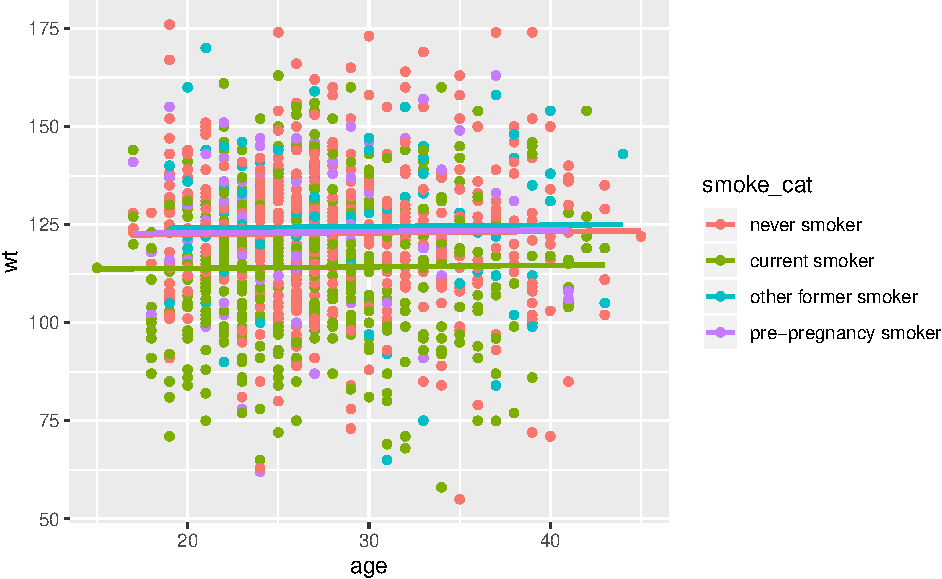
\includegraphics{10_Lab_Answers_files/figure-latex/unnamed-chunk-10-1.pdf}

\begin{Shaded}
\begin{Highlighting}[]
\NormalTok{smoke_cur_dage<-}\KeywordTok{lm}\NormalTok{(wt}\OperatorTok{~}\NormalTok{smoke_cur_d}\OperatorTok{+}\NormalTok{age, }\DataTypeTok{data=}\NormalTok{Gestation)}
\end{Highlighting}
\end{Shaded}

\begin{Shaded}
\begin{Highlighting}[]
\KeywordTok{qplot}\NormalTok{(}\DataTypeTok{y=}\NormalTok{wt, }\DataTypeTok{x=}\NormalTok{age, }\DataTypeTok{color=}\NormalTok{smoke_cur_d, }\DataTypeTok{data=}\NormalTok{Gestation)}\OperatorTok{+}\KeywordTok{geom_parallel_slopes}\NormalTok{(}\DataTypeTok{se=}\OtherTok{FALSE}\NormalTok{)}
\end{Highlighting}
\end{Shaded}

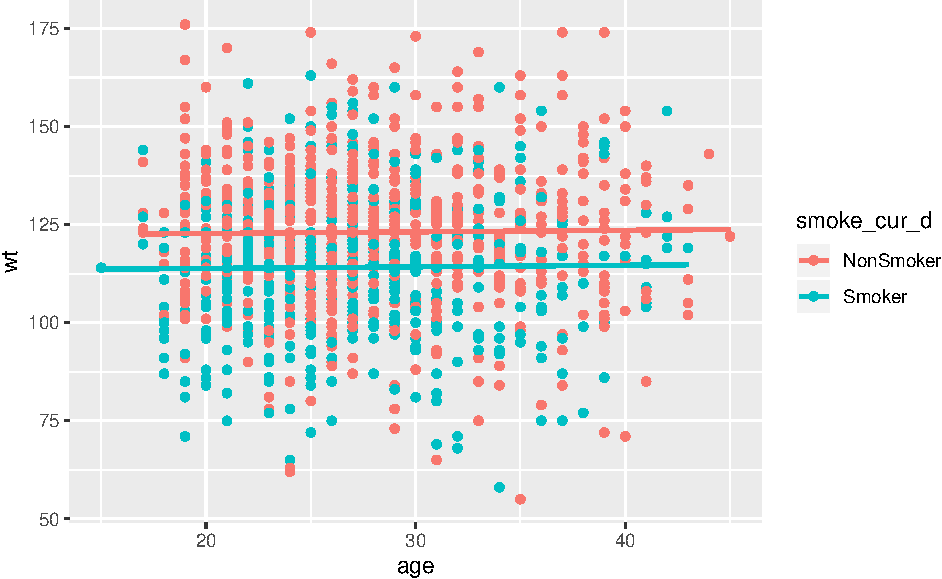
\includegraphics{10_Lab_Answers_files/figure-latex/unnamed-chunk-11-1.pdf}

\begin{Shaded}
\begin{Highlighting}[]
\NormalTok{wt4cat_temp<-}\KeywordTok{lm}\NormalTok{(wt}\OperatorTok{~}\NormalTok{smoke_cat}\OperatorTok{+}\NormalTok{age, }\DataTypeTok{data=}\NormalTok{Gestation)}
\end{Highlighting}
\end{Shaded}

\newpage

We are essentially testing the hypothesis that former smokers and quit
at pregnancy are the same as never smokers vs.~the alternative that one
of them is different.

\[H_0: \beta_\text{former} = \beta_\text{quit-at-pregancy} = 0 \]
\[H_A: \beta_i \neq 0 \]

\hypertarget{nested-model}{%
\subparagraph{Nested Model}\label{nested-model}}

\begin{Shaded}
\begin{Highlighting}[]
\KeywordTok{anova}\NormalTok{(smoke_cur_dage)}
\end{Highlighting}
\end{Shaded}

\begin{verbatim}
## Analysis of Variance Table
## 
## Response: wt
##               Df Sum Sq Mean Sq F value Pr(>F)    
## smoke_cur_d    1  23393 23392.7 74.6822 <2e-16 ***
## age            1     67    66.6  0.2126 0.6448    
## Residuals   1221 382454   313.2                   
## ---
## Signif. codes:  0 '***' 0.001 '**' 0.01 '*' 0.05 '.' 0.1 ' ' 1
\end{verbatim}

\hypertarget{full-model}{%
\subparagraph{Full Model}\label{full-model}}

\begin{Shaded}
\begin{Highlighting}[]
\KeywordTok{anova}\NormalTok{(wt4cat_temp)}
\end{Highlighting}
\end{Shaded}

\begin{verbatim}
## Analysis of Variance Table
## 
## Response: wt
##             Df Sum Sq Mean Sq F value    Pr(>F)    
## smoke_cat    3  23632  7877.2 25.1221 8.991e-16 ***
## age          1     58    57.9  0.1848    0.6674    
## Residuals 1219 382224   313.6                      
## ---
## Signif. codes:  0 '***' 0.001 '**' 0.01 '*' 0.05 '.' 0.1 ' ' 1
\end{verbatim}

\hypertarget{nested-f-test}{%
\subparagraph{Nested F Test}\label{nested-f-test}}

\begin{Shaded}
\begin{Highlighting}[]
\KeywordTok{anova}\NormalTok{(smoke_cur_dage, wt4cat_temp)}
\end{Highlighting}
\end{Shaded}

\begin{verbatim}
## Analysis of Variance Table
## 
## Model 1: wt ~ smoke_cur_d + age
## Model 2: wt ~ smoke_cat + age
##   Res.Df    RSS Df Sum of Sq     F Pr(>F)
## 1   1221 382454                          
## 2   1219 382224  2    230.14 0.367 0.6929
\end{verbatim}

The nested-F test is
\[Nested F = \frac{\frac{SSM_\text{full}-SSM_\text{nested}}{\text{Number of predictors}}}{\frac{SSE_\text{Full}}{n-k-1}}\]

In this case, we have
\(Nested F = \frac{\frac{23632-23393}{2}}{\frac{382224}{1219}} = \frac{\frac{230.14}{2}}{313.5} = \frac{115.07}{313.5} = 0.367\)

We fail to reject the null hypothesis (the F statistic is very small,
\textless{}1, and the p-value is very large and above our standard
threshold 0.69\textgreater{}0.05) and conclude that we don't have
evidence that former and quit-at-pregnancy aren't the same as each
other. Thus, a model with just non-smokers vs.~smokers does just as well
as a model with all four categories (current vs.~never, former,
quit-at-pregnancy).

\end{document}
